\documentclass[../main.tex]{subfiles}
\graphicspath{{\subfix{../Figures/}}}
\begin{document}
	
	\begin{frame}{Definitions}
		\begin{columns}
			\column{0.5\textwidth}
				Graph($n=10, m=9$)
				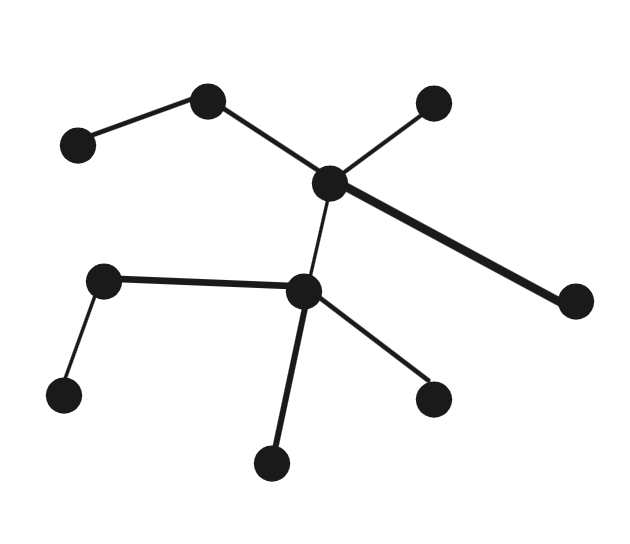
\includegraphics[width=1.0\textwidth]{Figures/graph}
			\column{0.5\textwidth}
				Hypergraph($n=10, m=3$)
				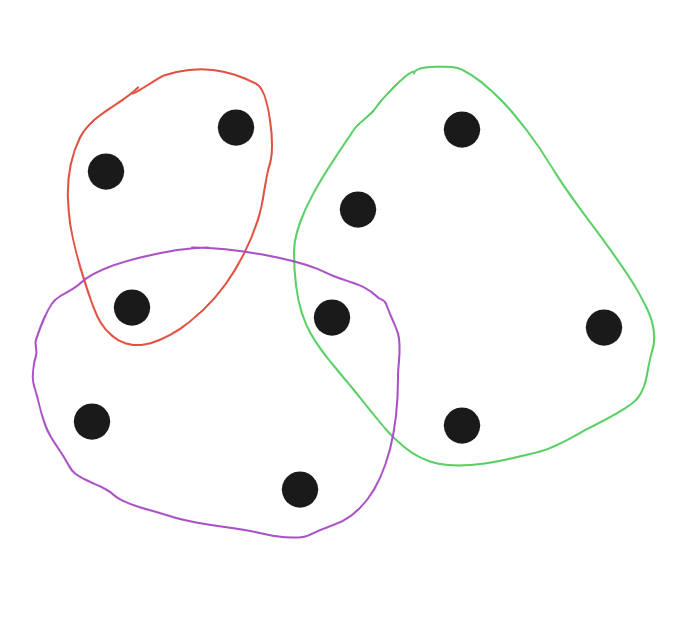
\includegraphics[width=1.0\textwidth]{hypergraph.png}
		\end{columns}
	\end{frame}

    \begin{frame}{Conductance} 
    	\begin{columns}
    		\column{0.5\textwidth}
				An interesting property of a graph is its conductance $\phi$:
	
	           	\begin{block}{Conductance}
	           		$\phi(S) = \frac{E(S, \bar{S})}{\min(\text{vol}(S), \text{vol}(\bar{S}))}$
	           	\end{block}
           		
           		The conductance of the cut $(S, \bar{S})$ in the figure is $\frac{1}{15z`}$
            \column{0.5\textwidth}
	            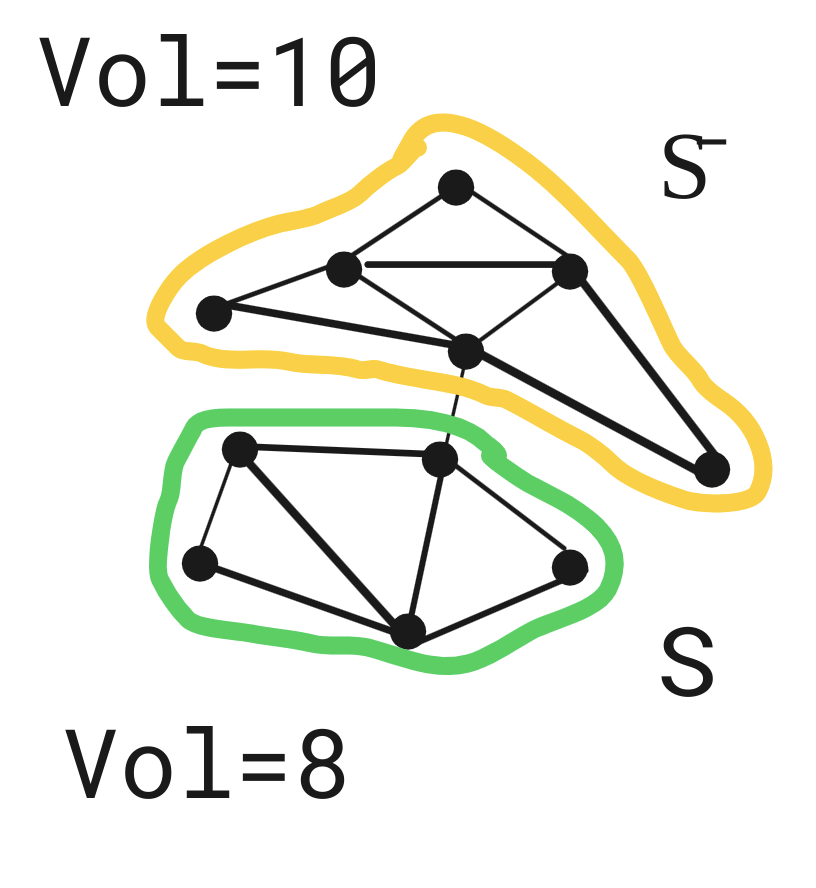
\includegraphics[width=1.0\textwidth]{conductance.png}
        \end{columns}
    \end{frame}

	\begin{frame}{Local Clustering}
		\begin{block}{Local Clustering Problem}
			Given a starting vertex $v$ and a target conductance $\hat{\phi}$, find a cut $S$ s.t. $v\in S$ and $\phi(S) \leq \hat{\phi}$. Must assume that $\exists S^*$ s.t. $v\in S^*$ and $\phi(S^*) \leq \frac{\hat{\phi}}{\log(n)} = \phi^*$.
		\end{block}
		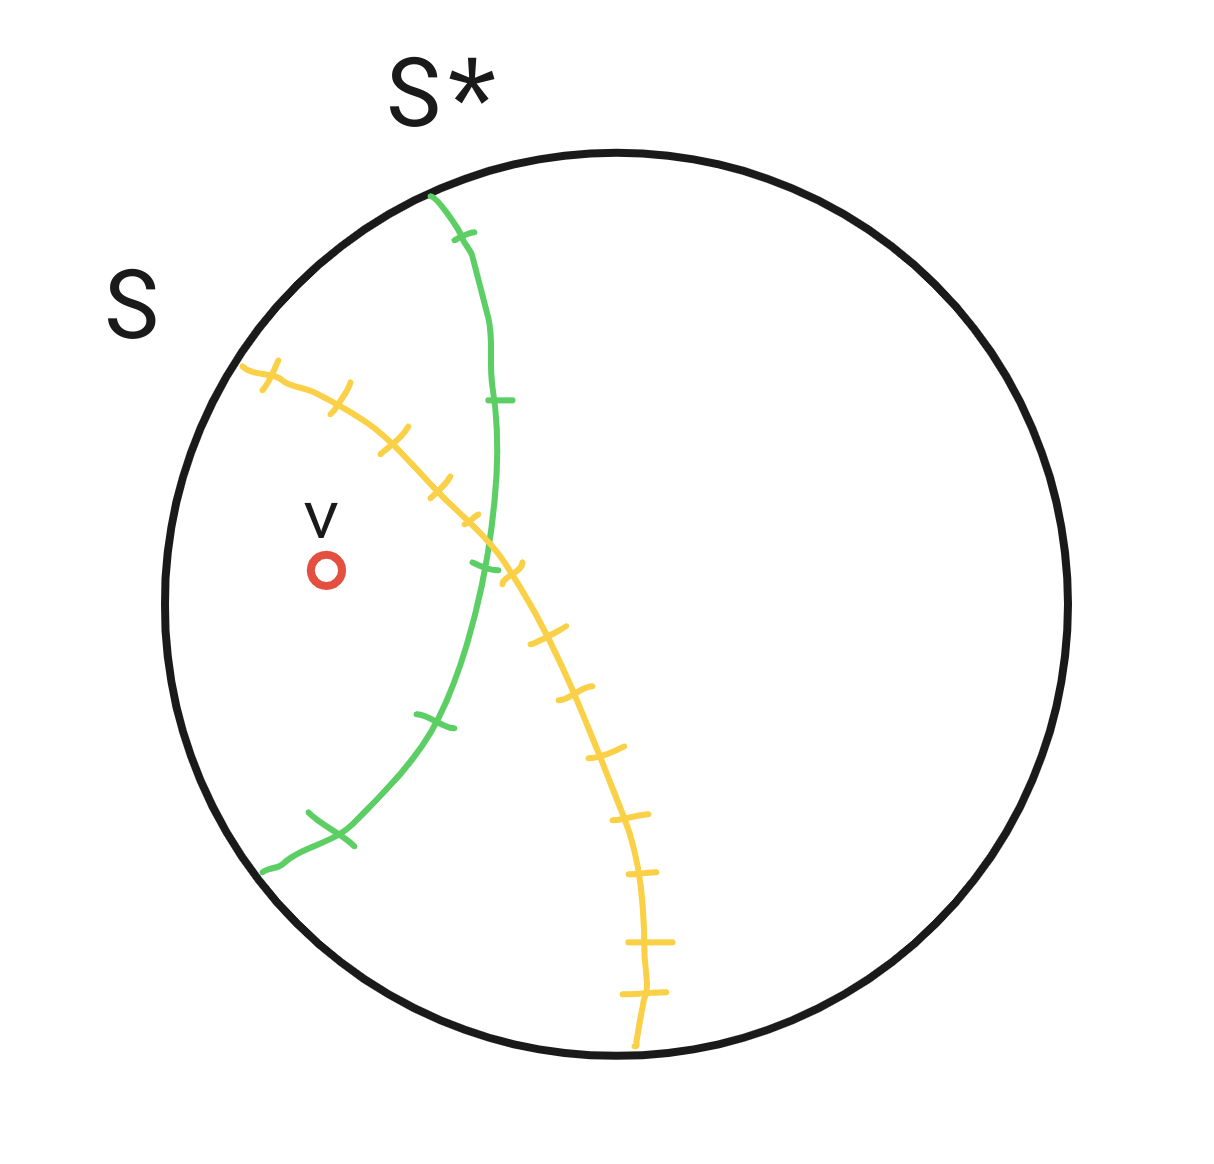
\includegraphics[width=0.5\textwidth]{local_clustering_algo_2}
	\end{frame}
    
    \begin{frame}{Random Walks in graphs}
    	\begin{columns}
    		\column{0.33\textwidth}
    			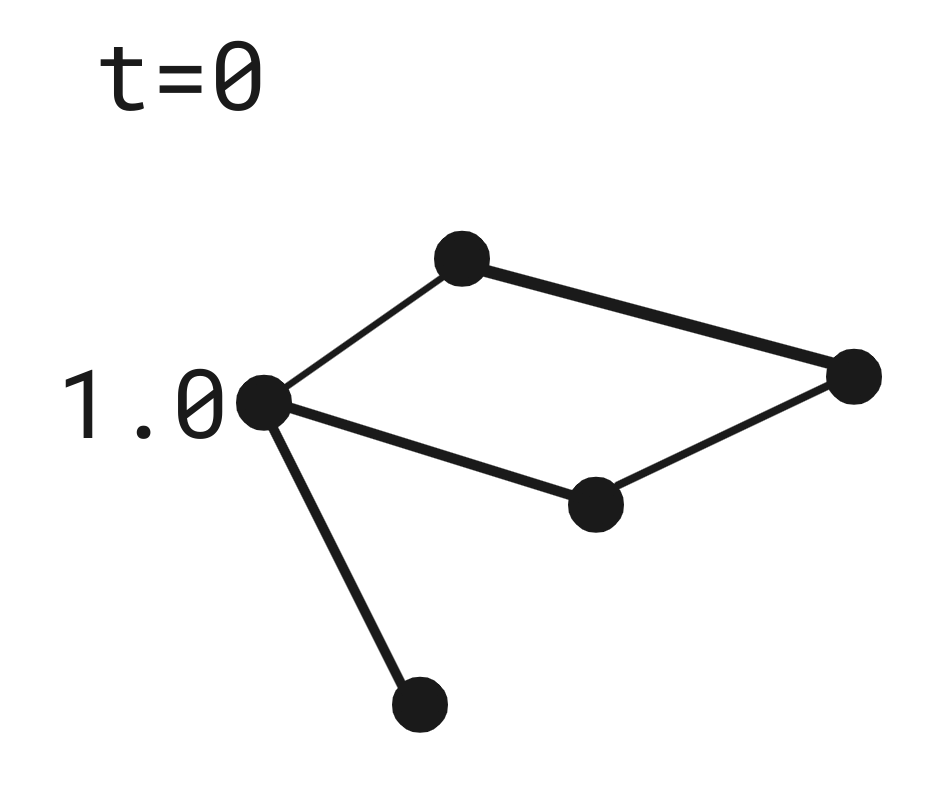
\includegraphics[width=1.\textwidth]{random_walk_t_0}
	   		\column{0.33\textwidth}
    			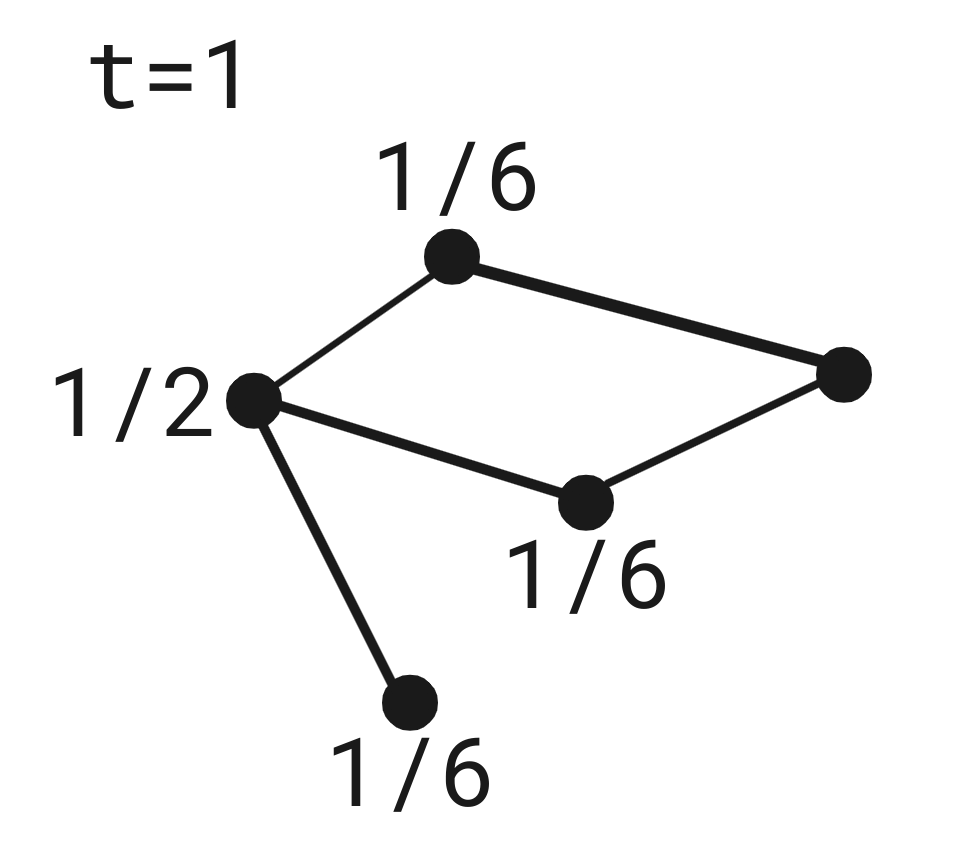
\includegraphics[width=1.\textwidth]{random_walk_t_1}
    		\column{0.33\textwidth}
    			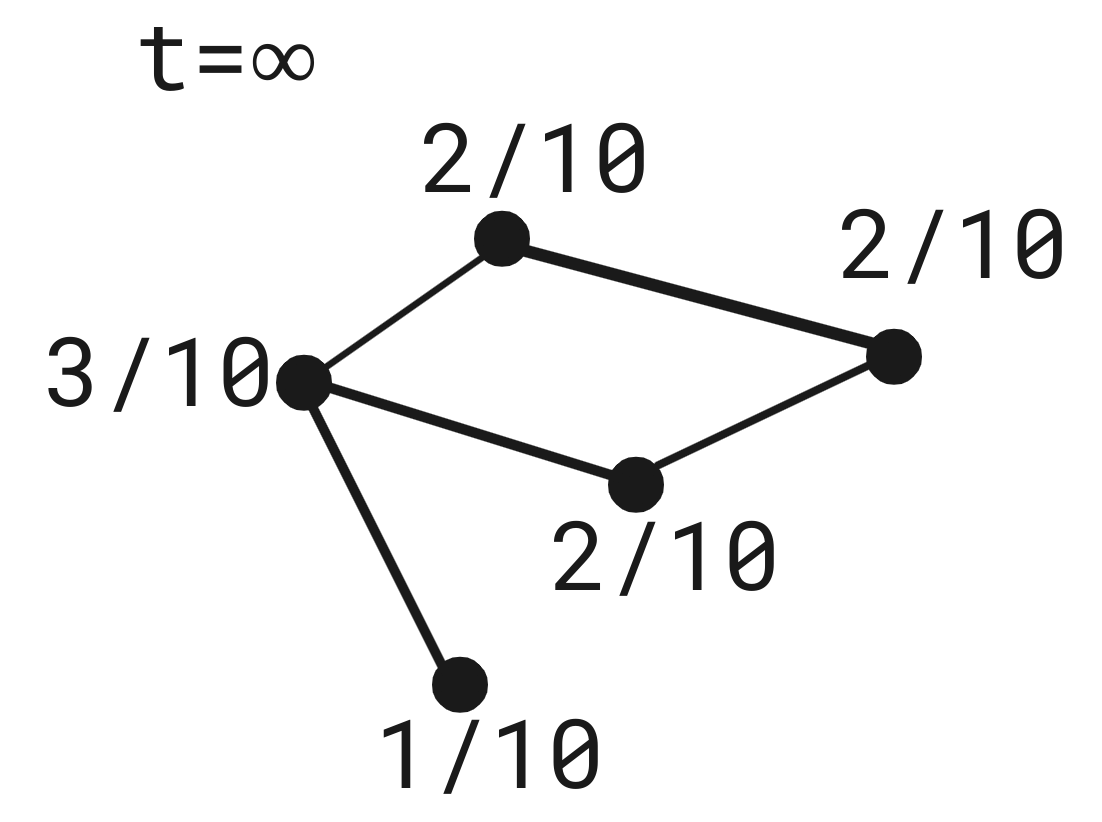
\includegraphics[width=1.0\textwidth]{random_walk_t_infinity}
    	\end{columns}
        
        Random walks are \textit{lazy} (w.p. $\frac{1}{2}$ you do not move)
            
        \begin{block}{Transition probability matrix}
            $p_{t+1} = \frac{1}{2}(I + AD^{-1}) p_t = M p_t$ 
        \end{block}
    
	    \begin{block}{Convergence to stationary distribution}
	    	when $t\to\infty \implies \bold{p}_t(u)\to \pi(u) = \frac{d(u)}{\text{vol}(G)}$
	    \end{block}
        
    \end{frame}
    
    
    \begin{frame}{Mixing}
           Studying how fast the probability vector converges to stationary distribution is called \textit{mixing}, and it is done with the Lovasz-Simonovits curve \cite{Lovsz1993RandomWI}.        
    \end{frame}
    
    \begin{frame}{Lovasz-Simonovits curve}
		\begin{columns}
 	    	\column{0.8\textwidth}
	        \begin{block}{Sweep Cut}
	            $S_j(\bold{p}_t)$: sort vertices by decreasing $\frac{p_t(u)}{d(u)}$ values, and take first $j$ vertices.
	        \end{block}
	    \end{columns}
    	\begin{columns}
    		\column{0.4\textwidth}
	    	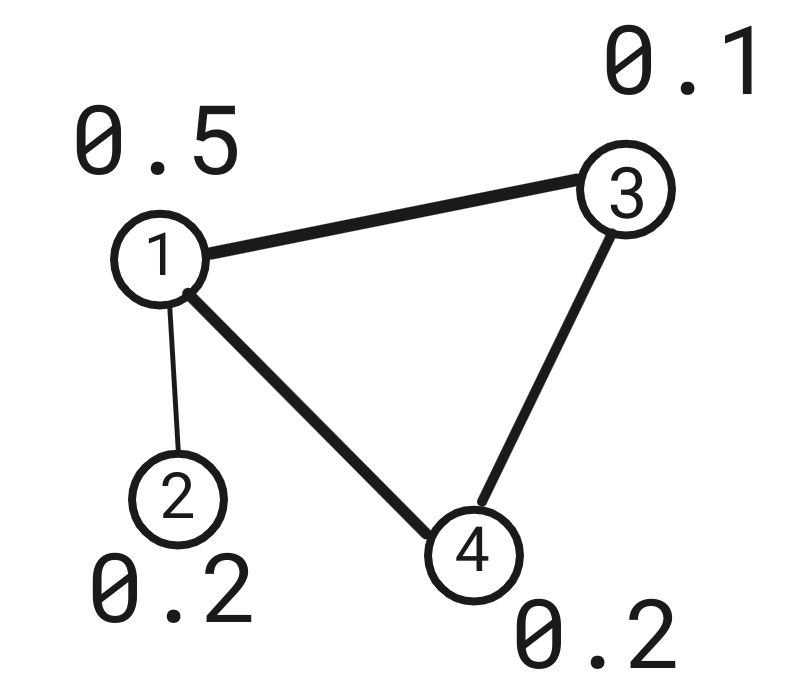
\includegraphics[width=0.8\textwidth]{lovasz_simonovits_graph}
	    	\column{0.8\textwidth}
	    	\begin{equation*}
	    		\text{sorted vertices} = [2, 1, 3, 4]
    		\end{equation*}
			\begin{equation*}
    			\text{volumes of sweep cuts} = [1, 4, 6, 8]
    		\end{equation*}
    		\begin{equation*}
    		\hspace*{-2cm}\text{probability mass on sweep cuts} = [0.2, 0.7, 0.9, 1.0]
    		\end{equation*}
    		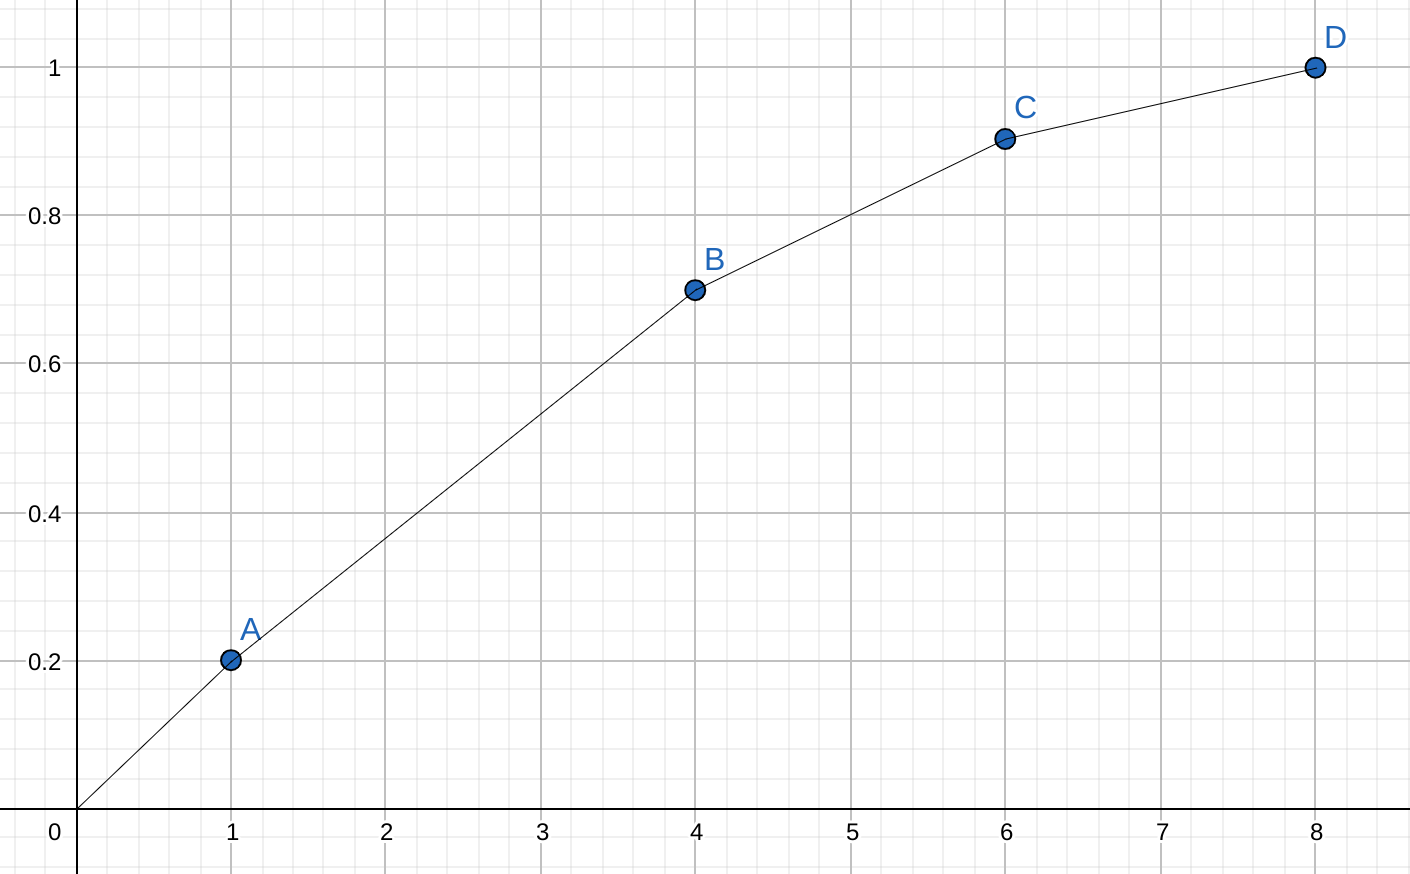
\includegraphics[width=0.6\textwidth]{ls_curve_test}
        \end{columns}
	\end{frame}
	
	\begin{frame}{Lovasz Simonovits Curve properties}
    
          	Properties: 
          	\begin{itemize}
          		\item concave
          		\item bounded in [0,1]
          		\item decreasing wrt time
          	\end{itemize}
     
         
     
		\begin{columns}
			\column{0.5\textwidth}
			\begin{block}{LS-curve is decreasing} 
				$I_{t+1}(k) \leq I_{t}(k)$
			\end{block}
	     	\column{0.5\textwidth}
		     	\raisebox{.0\height}{
		        	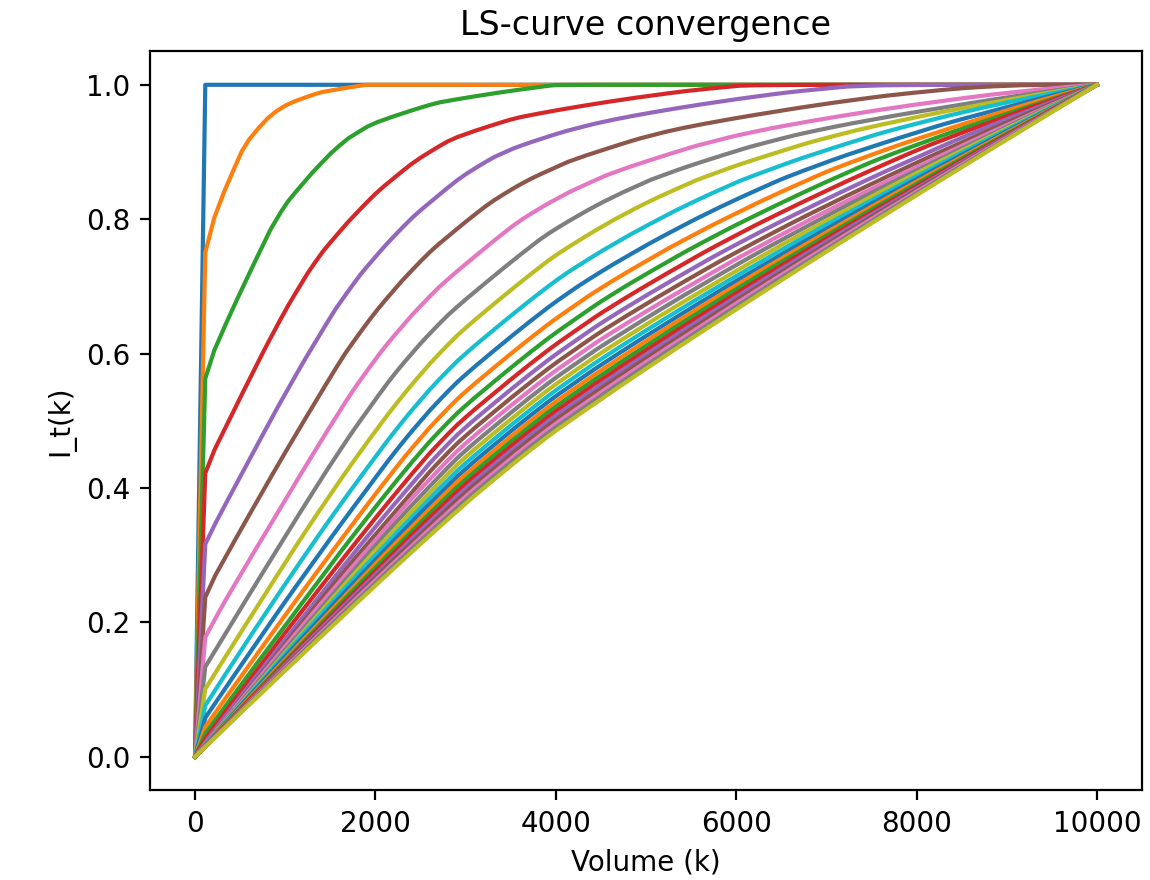
\includegraphics[width=0.9\textwidth]{LS-curve_convergence}
		       	}
    	\end{columns}
    \end{frame}
    
    \begin{frame}{1. Studying mixing with Lovasz-Simonovits curve}
        \begin{itemize}
            \item $\hat{\phi} = \min_{j\in[1,n]}\phi(S_j(\bold{p}_t))$ and $\hat{k}:=\min(k, \text{vol}(G)-k)$
                \begin{columns}
                    \column{0.5\textwidth}
                    \begin{block}{Recursive upper bound of LS curve}
                        $I_{t+1}(k) \leq \frac{1}{2}(I_t(k-\hat{\phi} \hat{k}) + I_t(k+\hat{\phi} \hat{k}))$
                    \end{block}
                	\column{0.5\textwidth}
                	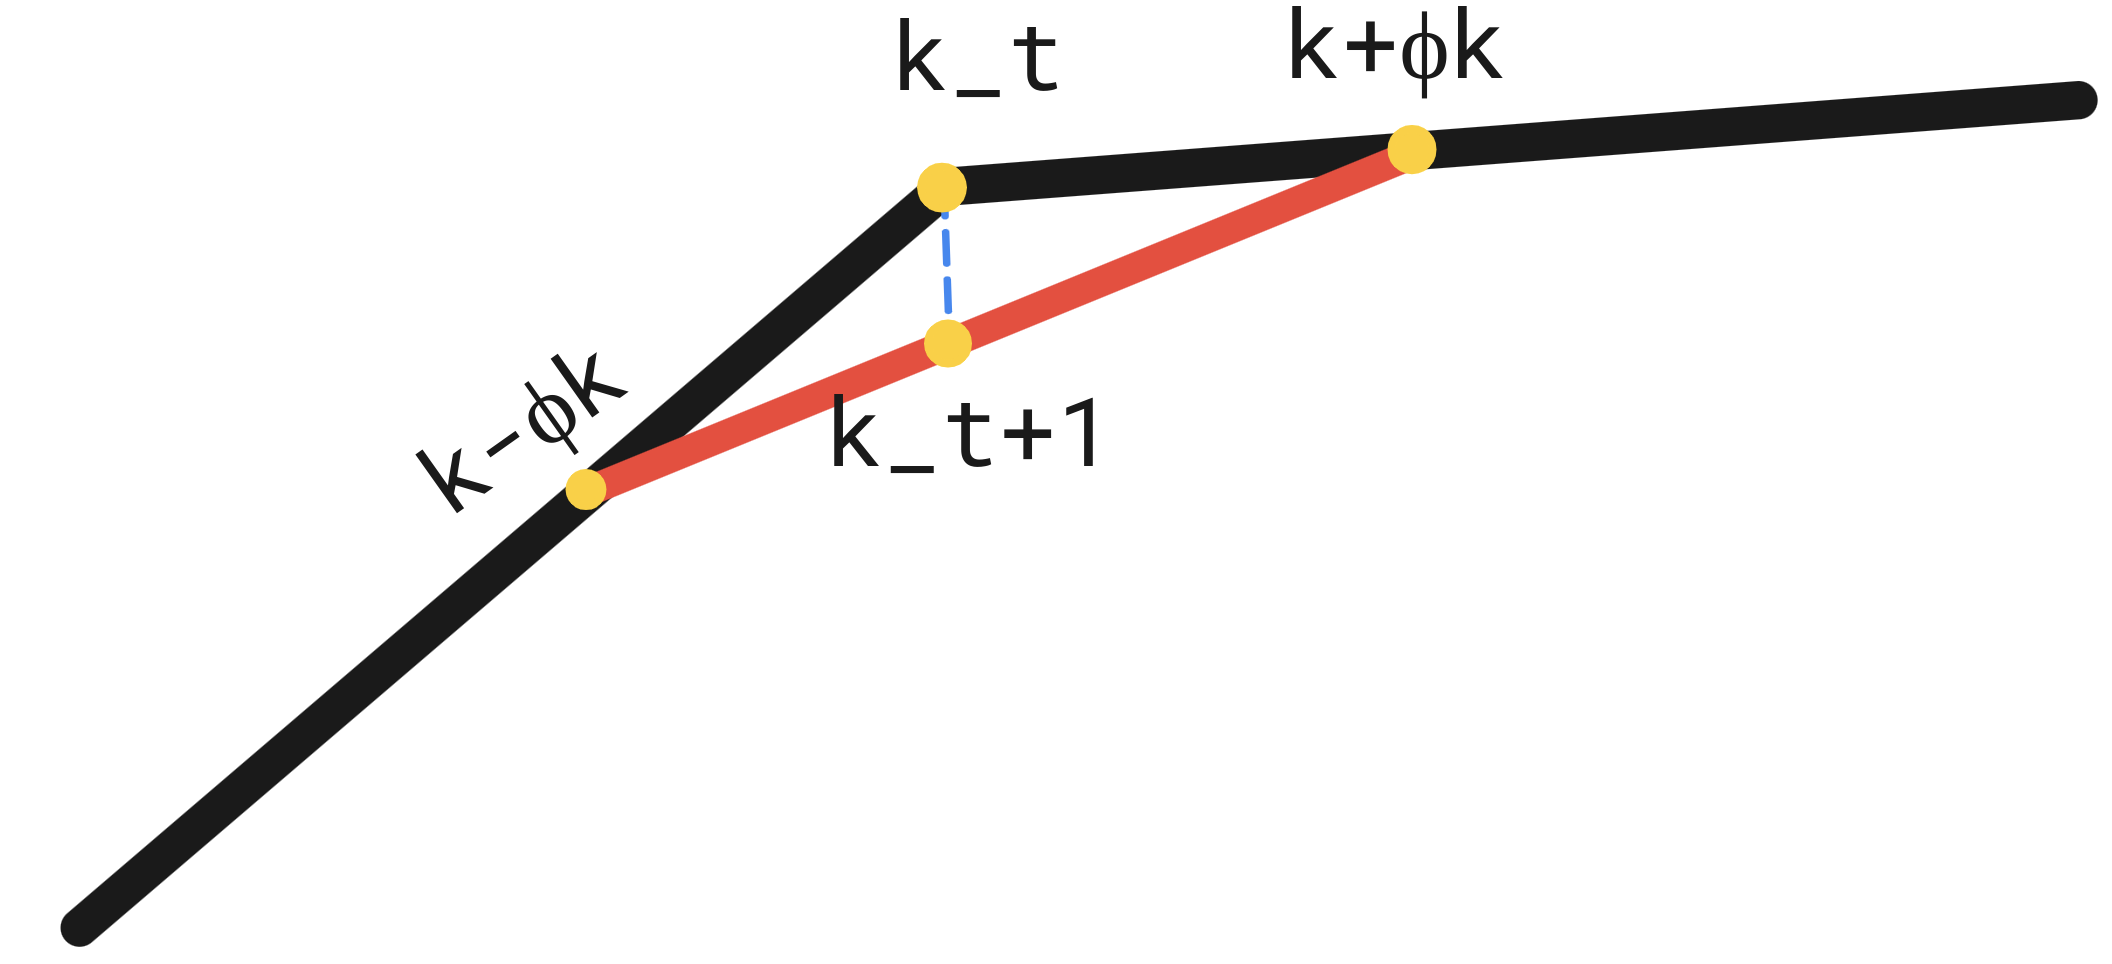
\includegraphics[width=1.\textwidth]{ls_recursive_upper_bound}
                \end{columns}
           \item This allows for exponentially fast convergence:
                \begin{columns}
                    \column{0.6\textwidth}
                    \begin{block}{Exponentially fast mixing wrt time}
                        $I_{t}(k) - \pi(S_j(\bold{p}_t)) \leq \sqrt{\hat{k}}e^{-t \hat{\phi}^2}$
                    \end{block}
                \end{columns}
        \end{itemize}
    \end{frame}
    
    \begin{frame}{Leaking of random walks in a graph}
        Leaking is the opposite of mixing: it says how slowly the random walk mixes.
        When $p_0= \psi_S$ for some $S\subseteq V$, then
        \begin{columns}
            \column{0.7\textwidth}
            \begin{block}{Leaking wrt optimal conductance $\phi^*$}
                $p_t(S) \geq 1 - t\phi(S)$
            \end{block}
        \end{columns}
            
            
        \begin{columns}
           	\column{0.33\textwidth}
           	\raisebox{-1.2\height}{
   	        	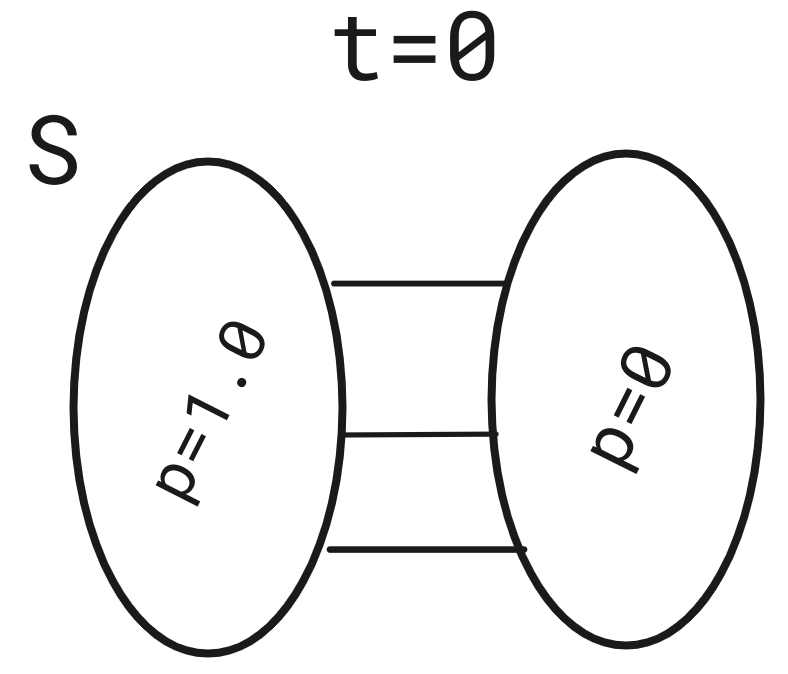
\includegraphics[width=1.0\textwidth]{leaking_t_0}}
           	\column{0.33\textwidth}
           	\raisebox{-1.2\height}{
				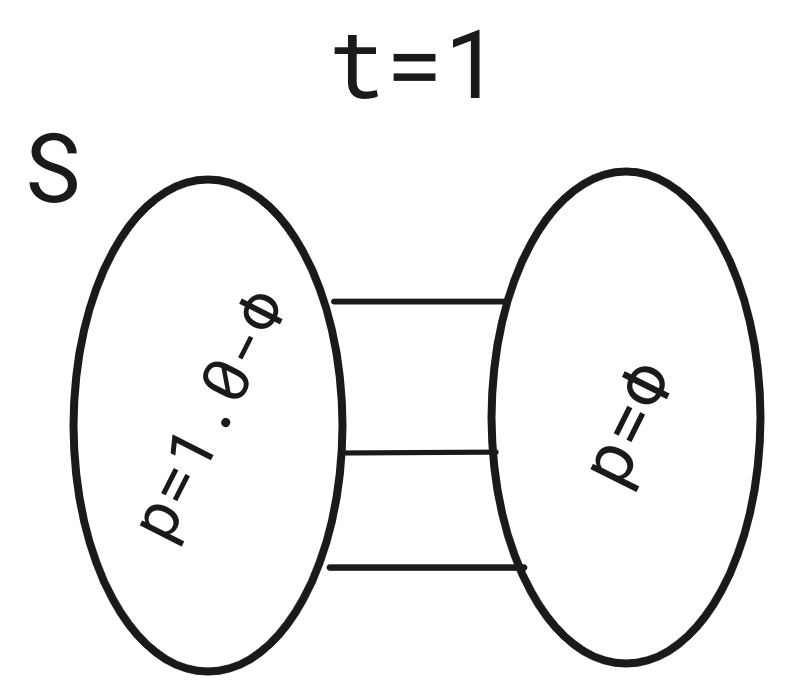
\includegraphics[width=1.0\textwidth]{leaking_t_1}}
           	\column{0.33\textwidth}
           	\raisebox{-1.2\height}{
				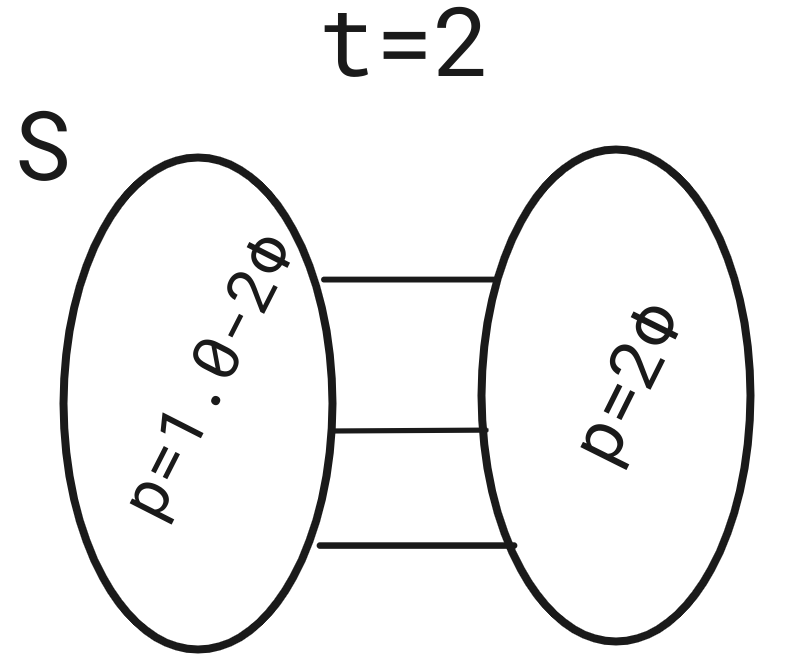
\includegraphics[width=1.0\textwidth]{leaking_t_2}}
	    \end{columns}
   \end{frame}
   
   	\begin{frame}{Leaking of random walks in a graph}
   		\begin{columns}
			\column{0.5\textwidth}
			Unfortunately, when starting with $p_0=\chi_v$ for some $v\in S$ the leaking result might not be true.
			\column{0.5\textwidth}
			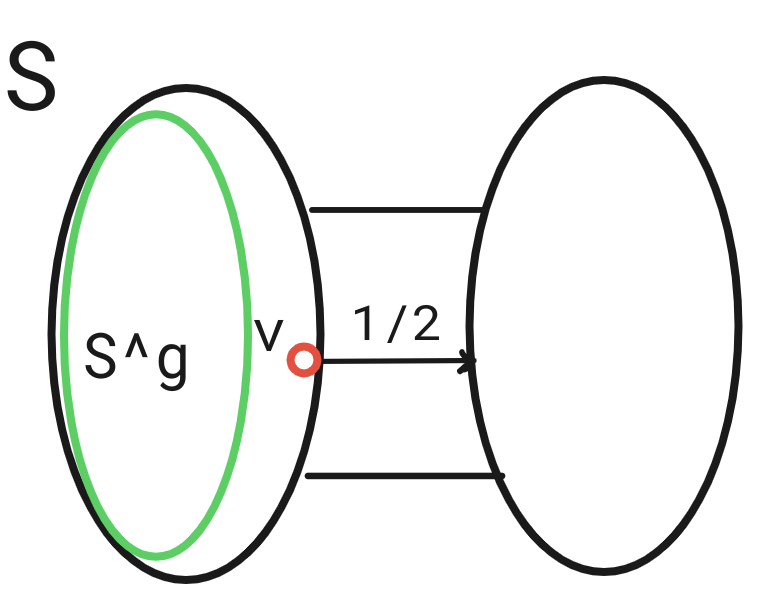
\includegraphics[width=0.8\textwidth]{leaking_v_bad}
		\end{columns}
		Luckily though, volume of these bad vertices $S^b$ for which the leaking result is not true is small: hence the volume of good vertices $S^g$ is large:
        \begin{columns}
            \column{0.7\textwidth}
            \begin{block}{Volume of $S^g$ is large}
                $\text{vol}(S^g) \geq \frac{1}{2}\text{vol}(S)$
            \end{block}
        \end{columns}
    \end{frame}
    
    \begin{frame}{Mixing+leaking = clustering algorithm}
            You pick a vertex $v$ at random according to the stationary distribution (with good probability it falls in $S^g$)
            
            \begin{columns}
            	\column{0.5\textwidth}
            	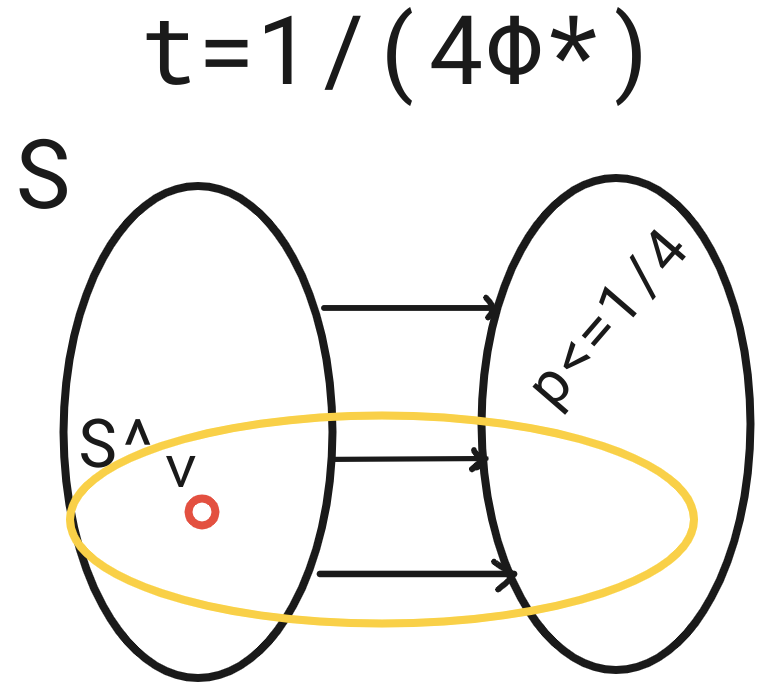
\includegraphics[width=0.8\textwidth]{local_clustering_algo_explain}
            	\column{0.5\textwidth}
            	\begin{equation*}
            	    \frac{1}{4} \leq p_t(S) - \pi(S) \leq \sqrt{\text{vol}(S)}e^{-t\hat{\phi}^2}
            	\end{equation*}
            	$\implies$
            	\begin{equation}
            		\hat{\phi} \leq \sqrt{\log(n) \phi^*}
            	\end{equation}
           	\end{columns}
           
            So the conductance of the output sweep cut $\phi(\hat{S}) = \hat{\phi}$ is \textit{not too far} from the optimal conductance $\phi(S) = \phi^*$ \cite{SpielmanClustering}.

    \end{frame}
    
    \begin{frame}{Local clustering algorithm for hypergraphs}
        \begin{itemize}
            \item In order to find a proper clustering algorithm for hypergraphs, we need to generalize both mixing and leaking results to hypergraphs. 
            \item Mixing: there have attempts to prove mixing using continuous diffusion processes \cite{Takai_2020}.
            \item Leaking: no known leaking result as far as we know.
        \end{itemize}
    \end{frame}
\end{document}